\documentclass[aspectratio=169,10pt]{beamer}

\usepackage[utf8]{inputenc}
\usepackage[T1]{fontenc}
\usepackage{lmodern}
\usepackage{amsmath,amssymb}
\usepackage{booktabs,tabularx,array,adjustbox}
\usepackage{tikz,pgfplots}
\usepackage[most]{tcolorbox}
\usepackage{graphicx,xcolor,ragged2e}
\pgfplotsset{compat=1.18}
\usetikzlibrary{arrows.meta,positioning,calc}

% ---------- Palette ----------
\definecolor{DeepNavy}{HTML}{073B4C}
\definecolor{Teal}{HTML}{118AB2}
\definecolor{SoftBlue}{HTML}{E8F4FA}
\definecolor{Orange}{HTML}{F26B21}
\definecolor{SoftOrange}{HTML}{FFF0E6}
\definecolor{Mint}{HTML}{D9F2EC}
\definecolor{Purple}{HTML}{6A4C93}
\definecolor{SoftPurple}{HTML}{F2ECFA}
\definecolor{Gold}{HTML}{F7B801}
\definecolor{SoftGold}{HTML}{FFF7D6}
\definecolor{GrayText}{HTML}{4A5568}
\definecolor{LightLine}{HTML}{D9E2EC}

% ---------- Beamer ----------
\setbeamertemplate{navigation symbols}{}
\setbeamercolor{normal text}{fg=DeepNavy,bg=white}
\setbeamercolor{frametitle}{fg=DeepNavy,bg=white}
\setbeamerfont{frametitle}{size=\Large,series=\bfseries}
\setbeamertemplate{frametitle}{%
  \vspace{0.25em}\insertframetitle\par
  \vspace{-0.25em}\tikz{\draw[Orange,line width=1.15pt] (0,0)--(1.15,0);}\vspace{-0.48em}
}
\setbeamertemplate{footline}{%
\leavevmode\hbox{%
\begin{beamercolorbox}[wd=.46\paperwidth,ht=2.2ex,dp=1ex,leftskip=1em]{}\scriptsize MA25-31017 Pemodelan Komputasi dan Analisis Numerik\end{beamercolorbox}%
\begin{beamercolorbox}[wd=.36\paperwidth,ht=2.2ex,dp=1ex,center]{}\scriptsize Program Studi Matematika ITERA\end{beamercolorbox}%
\begin{beamercolorbox}[wd=.18\paperwidth,ht=2.2ex,dp=1ex,rightskip=1em plus1fil]{}\scriptsize \insertframenumber/\inserttotalframenumber\end{beamercolorbox}}%
}

% ---------- Boxes ----------
\tcbset{enhanced,boxrule=.7pt,arc=2mm,left=2mm,right=2mm,top=1mm,bottom=1mm,fonttitle=\bfseries,before skip=1pt,after skip=1pt}
\newtcolorbox{bluebox}[1][]{colback=SoftBlue,colframe=Teal,title=#1}
\newtcolorbox{orangebox}[1][]{colback=SoftOrange,colframe=Orange,title=#1}
\newtcolorbox{greenbox}[1][]{colback=Mint,colframe=DeepNavy!55!Teal,title=#1}
\newtcolorbox{purplebox}[1][]{colback=SoftPurple,colframe=Purple,title=#1}
\newtcolorbox{goldbox}[1][]{colback=SoftGold,colframe=Gold!80!black,title=#1}
\newcommand{\highlight}[1]{\textcolor{Orange}{\textbf{#1}}}
\newcommand{\smallgray}[1]{\textcolor{GrayText}{\scriptsize #1}}
\newcommand{\excel}[1]{\texttt{\detokenize{#1}}}

\begin{document}

% ============ 1. COVER ============
\begin{frame}[plain]
\begin{tikzpicture}[remember picture,overlay]
  \fill[SoftBlue] (current page.north west) rectangle ([xshift=.48\paperwidth]current page.south west);
  \fill[white] ([xshift=.48\paperwidth]current page.north west) rectangle (current page.south east);
\end{tikzpicture}
\vspace{0.62cm}
\begin{columns}[T,totalwidth=\textwidth]
\begin{column}{.44\textwidth}
{\fontsize{21}{24}\selectfont\bfseries Pemodelan Komputasi\\dan Analisis Numerik}\par
\vspace{0.12cm}
\tikz{\draw[Orange,line width=1.5pt] (0,0)--(1.9,0);}\par
\vspace{0.15cm}
{\large SPL, SPNL, Regresi Linear,\\dan Pencocokan Kurva}\par
\vspace{0.40cm}
\small MA25-31017 \textbullet\ Pertemuan 2\par
\small Program Studi Matematika\par
\small Institut Teknologi Sumatera\par
\vspace{0.28cm}
\textbf{Dosen Pengampu}\par
Rifky Fauzi\par
Dear Michiko Mutiara Noor
\end{column}
\begin{column}{.52\textwidth}
\vspace{0.2cm}
\begin{tikzpicture}
\begin{axis}[width=\linewidth,height=.52\textheight,axis lines=middle,
  xmin=0,xmax=8,ymin=0,ymax=7,grid=both,grid style={LightLine!55},
  xlabel={$x$},ylabel={$y$},xtick={2,4,6},ytick={2,4,6},
  tick label style={font=\scriptsize},label style={font=\scriptsize}]
\addplot[only marks,mark=*,mark size=2pt,Teal] coordinates
  {(1,0.5) (2,2.5) (3,2.0) (4,4.0) (5,3.5) (6,6.0) (7,5.5)};
\addplot[Orange,very thick,domain=0.5:7.5]{0.07142857+0.83928571*x};
\node[font=\scriptsize,Orange,anchor=north west] at (axis cs:3.4,2.6) {$f(x)=a+bx$};
\end{axis}
\end{tikzpicture}
\par\vspace{-0.15cm}
\centering\smallgray{Dari data ke model: menentukan parameter secara numerik.}
\end{column}
\end{columns}
\end{frame}

% ============ 2. BENANG MERAH ============
\begin{frame}{Benang Merah: Semuanya Kembali ke $F(\mathbf{x})=\mathbf{0}$}
\scriptsize
\begin{bluebox}[Ingat Pertemuan 1]
Pencarian akar mencari $x$ sehingga $f(x)=0$: \textbf{tebak, evaluasi, perbaiki}, lalu ukur galat dan periksa konvergensi. Hari ini pola yang sama muncul kembali dalam dimensi yang lebih tinggi.
\end{bluebox}
\vspace{1mm}
\begin{columns}[T,totalwidth=\textwidth]
\begin{column}{.49\textwidth}
\begin{orangebox}[Empat topik dengan satu ide]
\begin{tabularx}{\linewidth}{>{\bfseries}p{.26\linewidth} X}
\toprule
Topik & Bentuk residual\\
\midrule
SPL & $A\mathbf{x}-\mathbf{b}=\mathbf{0}$\\
SPNL & $F(\mathbf{x})=\mathbf{0}$\\
Regresi linear & $\nabla S_r=\mathbf{0}\Rightarrow$ SPL normal\\
Curve fitting & $\nabla S_r=\mathbf{0}$, nonlinear\\
\bottomrule
\end{tabularx}
\end{orangebox}
\end{column}
\begin{column}{.47\textwidth}
\begin{greenbox}[Yang berulang sepanjang MK]
\begin{itemize}\setlength\itemsep{2pt}
\item \textbf{Iterasi}: tebakan awal diperbaiki bertahap.
\item \textbf{Galat}: $\varepsilon_a=\left|\frac{x^{(k)}-x^{(k-1)}}{x^{(k)}}\right|100\%$.
\item \textbf{Konvergensi}: kapan boleh berhenti, dan kapan justru divergen.
\end{itemize}
\end{greenbox}
\begin{goldbox}[Alur pertemuan ini]
\centering\textbf{SPL $\rightarrow$ SPNL $\rightarrow$ Regresi $\rightarrow$ Curve Fitting}
\end{goldbox}
\end{column}
\end{columns}
\end{frame}

% ============ 3. MOTIVASI SPL ============
\begin{frame}{Dari Hukum Konservasi Massa Menuju SPL}
\scriptsize
\begin{columns}[T,totalwidth=\textwidth]
\begin{column}{.50\textwidth}
\begin{adjustbox}{max width=\linewidth,center}
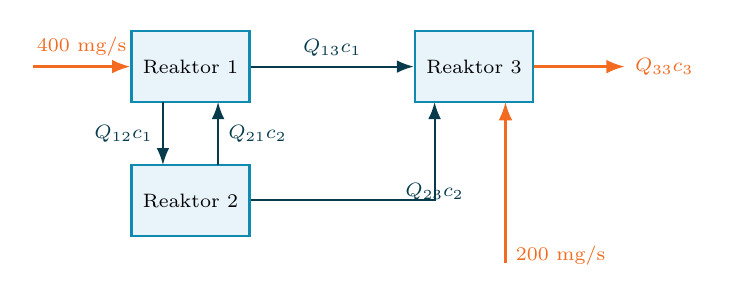
\begin{tikzpicture}[font=\scriptsize,>=Latex,line width=.7pt]
\node[draw=Teal,fill=SoftBlue,minimum width=1.5cm,minimum height=.9cm,line width=.8pt] (r1) at (0,1.7) {Reaktor 1};
\node[draw=Teal,fill=SoftBlue,minimum width=1.5cm,minimum height=.9cm,line width=.8pt] (r2) at (0,0) {Reaktor 2};
\node[draw=Teal,fill=SoftBlue,minimum width=1.5cm,minimum height=.9cm,line width=.8pt] (r3) at (3.6,1.7) {Reaktor 3};
% umpan luar
\draw[->,Orange,thick] (-2.0,1.7)--(r1.west) node[midway,above]{400 mg/s};
\draw[->,Orange,thick] (4.0,-0.8)--(4.0,1.25) node[pos=.05,right]{200 mg/s};
% keluaran
\draw[->,Orange,thick] (r3.east)--++(1.15,0) node[right]{$Q_{33}c_3$};
% antar reaktor
\draw[->,DeepNavy] (-0.35,1.25)--(-0.35,0.45) node[midway,left]{$Q_{12}c_1$};
\draw[->,DeepNavy] (0.35,0.45)--(0.35,1.25) node[midway,right]{$Q_{21}c_2$};
\draw[->,DeepNavy] (r1.east)--(r3.west) node[midway,above]{$Q_{13}c_1$};
\draw[->,DeepNavy] (r2.east)--(3.1,0)--(3.1,1.25) node[pos=.28,below]{$Q_{23}c_2$};
\end{tikzpicture}
\end{adjustbox}
\par\vspace{1mm}
\smallgray{Skema mengikuti Chapra \& Canale (2015): laju massa lewat pipa $=Q\cdot c$ dari arah aliran berasal.}
\end{column}
\begin{column}{.46\textwidth}
\begin{bluebox}[Neraca massa tiap reaktor]
Pada keadaan tunak, untuk setiap reaktor berlaku
\[
\sum(\text{massa masuk})=\sum(\text{massa keluar}).
\]
Satu reaktor menghasilkan satu persamaan; konsentrasi $c_1,c_2,c_3$ saling terkait.
\end{bluebox}
\begin{orangebox}[Hasilnya]
Sistem persamaan \textbf{linear} dalam $c_1,c_2,c_3$. Untuk jaringan besar (puluhan hingga ribuan simpul), penyelesaian manual tidak realistis.
\end{orangebox}
\begin{greenbox}[Contoh lain]
Rangkaian listrik, struktur rangka, diskretisasi PDB/PDE, dan persamaan normal pada regresi.
\end{greenbox}
\end{column}
\end{columns}
\end{frame}

% ============ 4. SPL FORMULASI ============
\begin{frame}{Sistem Persamaan Linear: Formulasi}
\scriptsize
\begin{columns}[T,totalwidth=\textwidth]
\begin{column}{.50\textwidth}
\begin{bluebox}[Bentuk umum]
\[
\begin{aligned}
a_{11}x_1+a_{12}x_2+\cdots+a_{1n}x_n&=b_1\\
a_{21}x_1+a_{22}x_2+\cdots+a_{2n}x_n&=b_2\\
&\;\;\vdots\\
a_{m1}x_1+a_{m2}x_2+\cdots+a_{mn}x_n&=b_m
\end{aligned}
\]
dengan $a_{ij},b_i\in\mathbb{R}$. Secara matriks:
\[
A\vec{x}=\vec{b}.
\]
\end{bluebox}
\end{column}
\begin{column}{.46\textwidth}
\begin{orangebox}[Dua keluarga metode]
\begin{tabularx}{\linewidth}{>{\bfseries}p{.24\linewidth} X}
\toprule
Langsung & Eliminasi Gauss, dekomposisi LU: solusi dalam langkah berhingga\\
Iteratif & Jacobi, Gauss-Seidel: barisan hampiran yang (semoga) konvergen\\
\bottomrule
\end{tabularx}
\end{orangebox}
\begin{greenbox}[Mengapa iteratif?]
Untuk matriks \textbf{besar dan jarang} (sparse), metode iteratif lebih hemat memori dan sering lebih cepat. Polanya juga persis metode pencarian akar: tebak, perbaiki, ukur galat.
\end{greenbox}
\end{column}
\end{columns}
\vfill
\smallgray{Fokus pertemuan ini: metode iteratif, sebagai jembatan menuju SPNL dan regresi.}
\end{frame}

% ============ 5. JACOBI ALGORITMA ============
\begin{frame}{Metode Jacobi: Algoritma}
\scriptsize
\begin{columns}[T,totalwidth=\textwidth]
\begin{column}{.53\textwidth}
\begin{bluebox}[Ide]
Isolasi $x_i$ dari persamaan ke-$i$, lalu hitung semua komponen \textbf{serentak} memakai nilai iterasi sebelumnya:
\[
x_i^{(k+1)}=\frac{b_i-\sum_{j\neq i}a_{ij}x_j^{(k)}}{a_{ii}},\quad i=1,\dots,n.
\]
Seluruh ruas kanan hanya memakai indeks $(k)$.
\end{bluebox}
\begin{orangebox}[Kriteria berhenti]
\[
|\varepsilon_{a,i}|=\left|\frac{x_i^{(k+1)}-x_i^{(k)}}{x_i^{(k+1)}}\right|100\%<\varepsilon_s
\]
untuk \textbf{semua} $i$; sediakan juga iterasi maksimum.
\end{orangebox}
\end{column}
\begin{column}{.43\textwidth}
\begin{greenbox}[Langkah]
\begin{enumerate}\setlength\itemsep{2pt}
\item Tetapkan toleransi $\varepsilon_s$.
\item Tetapkan tebakan awal, umumnya $x_i^{(0)}=0$.
\item Hitung seluruh $x_i^{(k+1)}$ dengan rumus di samping.
\item Hitung $|\varepsilon_{a,i}|$ tiap komponen.
\item Berhenti jika semua $|\varepsilon_{a,i}|<\varepsilon_s$; jika belum, kembali ke langkah 3.
\end{enumerate}
\end{greenbox}
\begin{goldbox}[Catatan]
Butuh $a_{ii}\neq0$. Bila ada diagonal nol, lakukan penukaran baris (pivoting) lebih dulu.
\end{goldbox}
\end{column}
\end{columns}
\end{frame}

% ============ 6. CONTOH JACOBI ============
\begin{frame}{Contoh Jacobi: Lengkapi Iterasi Berikutnya}
\tiny
\begin{columns}[T,totalwidth=\textwidth]
\begin{column}{.46\textwidth}
\begin{bluebox}[Sistem]
\[
\begin{aligned}
3x_1-0.1x_2-0.2x_3&=7.85\\
0.1x_1+7x_2-0.3x_3&=-19.3\\
0.3x_1-0.2x_2+10x_3&=71.4
\end{aligned}
\]
Target $\varepsilon_{a,i}<0.001\%$, mulai dari $x^{(0)}=\mathbf{0}$.
\end{bluebox}
\begin{orangebox}[Formula iteratif]
\[
\begin{aligned}
x_1^{(k+1)}&=\tfrac{7.85+0.1x_2^{(k)}+0.2x_3^{(k)}}{3}\\[1mm]
x_2^{(k+1)}&=\tfrac{-19.3-0.1x_1^{(k)}+0.3x_3^{(k)}}{7}\\[1mm]
x_3^{(k+1)}&=\tfrac{71.4-0.3x_1^{(k)}+0.2x_2^{(k)}}{10}
\end{aligned}
\]
\end{orangebox}
\end{column}
\begin{column}{.50\textwidth}
\renewcommand{\arraystretch}{1.16}
\begin{adjustbox}{max width=\linewidth,center}
\begin{tabular}{c c c c c}
\toprule
$k$ & $x_1^{(k)}$ & $x_2^{(k)}$ & $x_3^{(k)}$ & $\max|\varepsilon_{a,i}|$\\
\midrule
0 & 0 & 0 & 0 & --\\
1 & 2.61666667 & $-2.75714286$ & 7.14000000 & 100\%\\
2 & 3.00076190 & $-2.48852381$ & 7.00635714 & 12.800\%\\
3 & $\cdots$ & $\cdots$ & $\cdots$ & $\cdots$\\
4 & $\cdots$ & $\cdots$ & $\cdots$ & $\cdots$\\
\bottomrule
\end{tabular}
\end{adjustbox}
\vspace{1mm}
\begin{greenbox}[Aktivitas kelas]
Hitung iterasi 3 dan 4, lalu lanjutkan di Excel hingga toleransi tercapai. Bandingkan dengan solusi eksak $x=(3,\,-2.5,\,7)$.
\end{greenbox}
\begin{goldbox}[Perhatikan]
Iterasi 2 memakai \textbf{seluruh} nilai iterasi 1, termasuk $x_1^{(1)}$ yang sebenarnya sudah tersedia lebih dulu.
\end{goldbox}
\end{column}
\end{columns}
\end{frame}

% ============ 7. GAUSS-SEIDEL ============
\begin{frame}{Metode Gauss-Seidel: Pakai Informasi Terbaru}
\scriptsize
\begin{columns}[T,totalwidth=\textwidth]
\begin{column}{.53\textwidth}
\begin{bluebox}[Modifikasi dari Jacobi]
Begitu $x_1^{(k+1)}$ selesai dihitung, langsung pakai untuk menghitung $x_2^{(k+1)}$, dan seterusnya:
\[
x_i^{(k+1)}=\frac{b_i-\sum_{j<i}a_{ij}x_j^{(k+1)}-\sum_{j>i}a_{ij}x_j^{(k)}}{a_{ii}}.
\]
\end{bluebox}
\begin{orangebox}[Beda satu kata dan beda perilaku]
\begin{tabularx}{\linewidth}{>{\bfseries}p{.24\linewidth} X}
\toprule
Jacobi & semua komponen dari iterasi $(k)$ \\
Gauss-Seidel & komponen $j<i$ sudah dari iterasi $(k+1)$\\
\bottomrule
\end{tabularx}
\end{orangebox}
\end{column}
\begin{column}{.43\textwidth}
\begin{greenbox}[Konsekuensi praktis]
\begin{itemize}\setlength\itemsep{2pt}
\item Umumnya konvergen lebih cepat pada sistem yang sama.
\item Hanya perlu satu vektor kerja (hemat memori).
\item Hasilnya bergantung pada \textbf{urutan persamaan}; Jacobi tidak.
\end{itemize}
\end{greenbox}
\begin{goldbox}[Hubungan ke titik tetap]
Keduanya berbentuk $\mathbf{x}^{(k+1)}=G(\mathbf{x}^{(k)})$ --- versi berdimensi $n$ dari metode titik tetap di Pertemuan 1.
\end{goldbox}
\end{column}
\end{columns}
\end{frame}

% ============ 8. CONTOH GAUSS-SEIDEL ============
\begin{frame}{Contoh Gauss-Seidel: Sistem yang Sama}
\tiny
\begin{columns}[T,totalwidth=\textwidth]
\begin{column}{.44\textwidth}
\begin{bluebox}[Formula iteratif]
\[
\begin{aligned}
x_1^{(k+1)}&=\tfrac{7.85+0.1x_2^{(k)}+0.2x_3^{(k)}}{3}\\[1mm]
x_2^{(k+1)}&=\tfrac{-19.3-0.1\highlight{$x_1^{(k+1)}$}+0.3x_3^{(k)}}{7}\\[1mm]
x_3^{(k+1)}&=\tfrac{71.4-0.3\highlight{$x_1^{(k+1)}$}+0.2\highlight{$x_2^{(k+1)}$}}{10}
\end{aligned}
\]
Yang berwarna adalah nilai yang \emph{baru saja} dihitung.
\end{bluebox}
\begin{orangebox}[Iterasi 1 secara rinci]
\[
\begin{aligned}
x_1^{(1)}&=\tfrac{7.85+0.1(0)+0.2(0)}{3}=2.6166667\\[1mm]
x_2^{(1)}&=\tfrac{-19.3-0.1(2.6167)+0.3(0)}{7}=-2.7945238\\[1mm]
x_3^{(1)}&=\tfrac{71.4-0.3(2.6167)+0.2(-2.7945)}{10}=7.0056095
\end{aligned}
\]
\smallgray{Nilai di dalam kurung dibulatkan agar muat; perhitungan tetap memakai presisi penuh.}
\end{orangebox}
\end{column}
\begin{column}{.52\textwidth}
\renewcommand{\arraystretch}{1.16}
\begin{adjustbox}{max width=\linewidth,center}
\begin{tabular}{c c c c c}
\toprule
$k$ & $x_1^{(k)}$ & $x_2^{(k)}$ & $x_3^{(k)}$ & $\max|\varepsilon_{a,i}|$\\
\midrule
0 & 0 & 0 & 0 & --\\
1 & 2.61666667 & $-2.79452381$ & 7.00560952 & 100\%\\
2 & $\cdots$ & $\cdots$ & $\cdots$ & $\cdots$\\
3 & $\cdots$ & $\cdots$ & $\cdots$ & $\cdots$\\
\bottomrule
\end{tabular}
\end{adjustbox}
\vspace{1mm}
\begin{greenbox}[Aktivitas kelas]
Lengkapi iterasi 2 dan 3, lalu bandingkan jumlah iterasi Gauss-Seidel dengan Jacobi untuk mencapai $\varepsilon_s$ yang sama. Sajikan plot $\varepsilon_a$ terhadap iterasi seperti pada Pertemuan 1.
\end{greenbox}
\begin{goldbox}[Diskusi]
Apakah percepatan ini berlaku untuk semua sistem, atau hanya untuk kelas matriks tertentu?
\end{goldbox}
\end{column}
\end{columns}
\end{frame}

% ============ 9. KONVERGENSI SPL ============
\begin{frame}{Kapan Metode Iteratif untuk SPL Konvergen?}
\scriptsize
\begin{columns}[T,totalwidth=\textwidth]
\begin{column}{.50\textwidth}
\begin{bluebox}[Syarat cukup yang mudah dipakai]
Matriks \textbf{dominan diagonal secara tegas}:
\[
|a_{ii}|>\sum_{j\neq i}|a_{ij}|\quad\text{untuk setiap }i.
\]
Jika terpenuhi, Jacobi dan Gauss-Seidel dijamin konvergen dari sebarang tebakan awal.
\end{bluebox}
\begin{orangebox}[Perhatikan arah implikasinya]
Ini syarat \textbf{cukup}, bukan syarat perlu. Sistem yang gagal memenuhinya masih mungkin konvergen; yang tidak dijamin hanyalah jaminannya.
\end{orangebox}
\end{column}
\begin{column}{.46\textwidth}
\begin{greenbox}[Rumusan matriks]
Tulis $\mathbf{x}^{(k+1)}=T\mathbf{x}^{(k)}+\mathbf{c}$. Barisan konvergen jika dan hanya jika radius spektral
\[
\rho(T)=\max_i|\lambda_i(T)|<1,
\]
dan makin kecil $\rho(T)$, makin cepat konvergensinya.
\end{greenbox}
\begin{goldbox}[Analogi Pertemuan 1]
Persis syarat $|g'(x)|<1$ pada metode titik tetap. $\rho(T)$ adalah versi matriksnya.
\end{goldbox}
\end{column}
\end{columns}
\vfill
\smallgray{Latihan: periksa dominansi diagonal sistem pada dua slide sebelumnya, lalu hitung $\rho(T)$ untuk Jacobi dan Gauss-Seidel.}
\end{frame}

% ============ 10. SPNL FORMULASI ============
\begin{frame}{Sistem Persamaan Nonlinear}
\scriptsize
\begin{columns}[T,totalwidth=\textwidth]
\begin{column}{.49\textwidth}
\begin{bluebox}[Bentuk umum]
\[
\begin{aligned}
f_1(x_1,x_2,\dots,x_n)&=0\\
f_2(x_1,x_2,\dots,x_n)&=0\\
&\;\;\vdots\\
f_m(x_1,x_2,\dots,x_n)&=0
\end{aligned}
\]
dengan setidaknya satu $f_i$ bukan fungsi linear. Ringkasnya $F(\mathbf{x})=\mathbf{0}$.
\end{bluebox}
\begin{orangebox}[Contoh]
\[
\begin{aligned}
x_1x_2+x_2^2x_3+x_3^2+2&=0\\
x_1^2+x_2x_3^2+x_2^2+3&=0\\
x_1x_3+x_2x_3^2+x_3^2+4&=0
\end{aligned}
\]
\end{orangebox}
\end{column}
\begin{column}{.47\textwidth}
\begin{greenbox}[Apa yang hilang dibanding SPL]
\begin{itemize}\setlength\itemsep{2pt}
\item Tidak ada rumus tertutup seperti eliminasi Gauss.
\item Solusi bisa \textbf{tidak ada, tunggal, atau banyak}.
\item Konvergensi bergantung kuat pada tebakan awal.
\end{itemize}
\end{greenbox}
\begin{goldbox}[Strateginya]
Gunakan kembali gagasan Newton-Raphson: dekati fungsi dengan model linear di sekitar tebakan, selesaikan model linear itu, lalu ulangi. Model linear tersebut berbentuk \textbf{SPL}.
\end{goldbox}
\end{column}
\end{columns}
\end{frame}

% ============ 11. MOTIVASI AI ============
\begin{frame}{Masalah Nonlinear di Kecerdasan Buatan}
\tiny
\begin{columns}[T,totalwidth=\textwidth]
\begin{column}{.49\textwidth}
\begin{bluebox}[Satu neuron dengan aktivasi sigmoid]
\[
\sigma(z)=\frac{1}{1+e^{-z}},\qquad y=\sigma(wx+b),
\]
dengan $w$ bobot dan $b$ bias. Diberikan tiga data latih
\[
(0,\,0.1),\quad(1,\,0.9),\quad(1.5,\,0.8).
\]
\end{bluebox}
\begin{orangebox}[Agar model ``belajar'']
Dicari $w$ dan $b$ sehingga
\[
\left\{
\begin{aligned}
\sigma(b)&=0.1\\
\sigma(w+b)&=0.9\\
\sigma(1.5w+b)&=0.8
\end{aligned}\right.
\]
Sistem ini nonlinear karena kehadiran $\sigma$.
\end{orangebox}
\end{column}
\begin{column}{.47\textwidth}
\begin{greenbox}[Bentuk residual]
\[
F(b,w)=
\begin{bmatrix}
\sigma(b)-0.1\\
\sigma(w+b)-0.9\\
\sigma(1.5w+b)-0.8
\end{bmatrix}=\vec{0}.
\]
\end{greenbox}
\begin{purplebox}[Perhatikan]
Ada \textbf{3 persamaan} tetapi hanya \textbf{2 parameter}. Sistem seperti ini umumnya tidak punya solusi eksak, sehingga yang dicari adalah parameter yang \textbf{memperkecil} $\|F\|$ --- inilah pintu masuk ke regresi nonlinear dan Gauss-Newton di paruh kedua pertemuan.
\end{purplebox}
\begin{goldbox}[Kaitan project]
Pelatihan model data-driven pada dasarnya penyelesaian sistem nonlinear berdimensi besar secara iteratif.
\end{goldbox}
\end{column}
\end{columns}
\end{frame}

% ============ 12. DERET TAYLOR ============
\begin{frame}{Linearisasi dengan Deret Taylor}
\scriptsize
\begin{bluebox}[Ekspansi orde satu untuk fungsi banyak variabel]
\[
f_i(x_1+\Delta x_1,\dots,x_n+\Delta x_n)\approx f_i(x_1,\dots,x_n)+\Delta x_1\frac{\partial f_i}{\partial x_1}+\Delta x_2\frac{\partial f_i}{\partial x_2}+\cdots+\Delta x_n\frac{\partial f_i}{\partial x_n}.
\]
\end{bluebox}
\vspace{1mm}
\begin{columns}[T,totalwidth=\textwidth]
\begin{column}{.50\textwidth}
\begin{orangebox}[Syaratkan langkah menuju solusi]
Jika $\mathbf{x}+\Delta\mathbf{x}$ adalah solusi, ruas kiri bernilai nol, sehingga
\[
-f_i(\mathbf{x})=\sum_{j=1}^{n}\Delta x_j\frac{\partial f_i}{\partial x_j},\quad i=1,\dots,m.
\]
\end{orangebox}
\end{column}
\begin{column}{.46\textwidth}
\begin{greenbox}[Yang kita peroleh]
Persamaan di samping \textbf{linear dalam $\Delta x_j$}. Masalah nonlinear berubah menjadi barisan masalah linear --- persis seperti Newton-Raphson satu variabel yang mengganti kurva dengan garis singgung.
\end{greenbox}
\begin{goldbox}[Harga yang dibayar]
Aproksimasi ini hanya baik di sekitar $\mathbf{x}$, sehingga langkahnya harus diulang dan tebakan awal tetap menentukan.
\end{goldbox}
\end{column}
\end{columns}
\end{frame}

% ============ 13. SPL DARI TAYLOR ============
\begin{frame}{SPL dari Deret Taylor: Matriks Jacobi}
\scriptsize
\begin{columns}[T,totalwidth=\textwidth]
\begin{column}{.56\textwidth}
\[
\underbrace{\begin{bmatrix}
\frac{\partial f_1}{\partial x_1} & \frac{\partial f_1}{\partial x_2} & \cdots & \frac{\partial f_1}{\partial x_n}\\[1mm]
\frac{\partial f_2}{\partial x_1} & \frac{\partial f_2}{\partial x_2} & \cdots & \frac{\partial f_2}{\partial x_n}\\[1mm]
\vdots & \vdots & \ddots & \vdots\\[1mm]
\frac{\partial f_m}{\partial x_1} & \frac{\partial f_m}{\partial x_2} & \cdots & \frac{\partial f_m}{\partial x_n}
\end{bmatrix}}_{A\ (\text{matriks Jacobi})}
\underbrace{\begin{bmatrix}\Delta x_1\\ \Delta x_2\\ \vdots\\ \Delta x_n\end{bmatrix}}_{\Delta X}
=
\underbrace{\begin{bmatrix}-f_1\\ -f_2\\ \vdots\\ -f_m\end{bmatrix}}_{-f}
\]
\begin{center}
\highlight{$A\,\Delta X=-f$}
\end{center}
\end{column}
\begin{column}{.40\textwidth}
\begin{bluebox}[Skema iterasi]
Pada langkah ke-$n$:
\begin{enumerate}\setlength\itemsep{2pt}
\item Susun $A^n$ dan $f^n$ di titik $\mathbf{x}^n$.
\item Selesaikan SPL $A^n\Delta X^n=-f^n$.
\item Perbarui
\[
x_i^{n+1}=x_i^n+\Delta x_i^n.
\]
\item Ulangi sampai
\[
\frac{|x_i^{n+1}-x_i^{n}|}{|x_i^{n+1}|}<\varepsilon_a .
\]
\end{enumerate}
\end{bluebox}
\begin{goldbox}[Inilah alasan urutannya]
SPL dipelajari lebih dulu karena \textbf{setiap} langkah SPNL adalah satu penyelesaian SPL.
\end{goldbox}
\end{column}
\end{columns}
\end{frame}

% ============ 14. CONTOH SPNL ============
\begin{frame}{Contoh SPNL: Iterasi Pertama}
\tiny
\begin{columns}[T,totalwidth=\textwidth]
\begin{column}{.50\textwidth}
\begin{bluebox}[Sistem dan turunan parsialnya]
\[
\begin{aligned}
f_1&=x_1x_2+x_2^2x_3+x_3^2+2\\
f_2&=x_1^2+x_2x_3^2+x_2^2+3\\
f_3&=x_1x_3+x_2x_3^2+x_3^2+4
\end{aligned}
\]
\[
A=\begin{bmatrix}
x_2 & x_1+2x_2x_3 & x_2^2+2x_3\\
2x_1 & x_3^2+2x_2 & 2x_2x_3\\
x_3 & x_3^2 & x_1+2x_2x_3+2x_3
\end{bmatrix}
\]
\end{bluebox}
\begin{orangebox}[Tebakan awal]
$x_1^0=x_2^0=x_3^0=1$, sehingga
\[
A^0=\begin{bmatrix}1&3&3\\2&3&2\\1&1&5\end{bmatrix},\qquad
-f^0=\begin{bmatrix}-5\\-6\\-7\end{bmatrix}.
\]
\end{orangebox}
\end{column}
\begin{column}{.46\textwidth}
\begin{greenbox}[Selesaikan SPL-nya]
\[
\begin{bmatrix}1&3&3\\2&3&2\\1&1&5\end{bmatrix}
\begin{bmatrix}\Delta x_1^0\\ \Delta x_2^0\\ \Delta x_3^0\end{bmatrix}
=\begin{bmatrix}-5\\-6\\-7\end{bmatrix}
\Rightarrow
\begin{bmatrix}\Delta x_1^0\\ \Delta x_2^0\\ \Delta x_3^0\end{bmatrix}
=\begin{bmatrix}-2\\ 0\\ -1\end{bmatrix}
\]
\end{greenbox}
\begin{purplebox}[Perbarui]
\[
\begin{bmatrix}x_1^1\\ x_2^1\\ x_3^1\end{bmatrix}
=\begin{bmatrix}1\\1\\1\end{bmatrix}+\begin{bmatrix}-2\\0\\-1\end{bmatrix}
=\begin{bmatrix}-1\\ 1\\ 0\end{bmatrix}
\]
\end{purplebox}
\begin{goldbox}[Aktivitas kelas]
Lakukan iterasi ke-2: susun $A^1$ dan $f^1$ di $\mathbf{x}^1=(-1,1,0)$, selesaikan SPL-nya, lalu hitung $\varepsilon_a$ tiap komponen. Perhatikan apakah $A^1$ masih taksingular.
\end{goldbox}
\end{column}
\end{columns}
\end{frame}

% ============ 15. PENCOCOKAN KURVA ============
\begin{frame}{Pencocokan Kurva: Model Menghampiri Data}
\scriptsize
\begin{columns}[T,totalwidth=\textwidth]
\begin{column}{.47\textwidth}
\begin{bluebox}[Model kandidat]
Linear:\quad $f(x)=a+bx$\par\vspace{1mm}
Polinom:\quad $f(x)=a_0+a_1x+a_2x^2+\cdots+a_nx^n$
\end{bluebox}
\begin{orangebox}[Data selalu memuat ketidakpastian]
Kesalahan model pada tiap titik didefinisikan
\[
e_i=y_i-f(x_i).
\]
Koefisien model dipilih agar kumpulan $e_i$ ini \textbf{kecil} menurut ukuran tertentu: rata-rata absolut, rata-rata kuadrat, dan seterusnya.
\end{orangebox}
\end{column}
\begin{column}{.49\textwidth}

\begin{tikzpicture}
\begin{axis}[width=\linewidth,height=.50\textheight,axis lines=middle,
  xmin=0,xmax=8,ymin=0,ymax=7,grid=both,grid style={LightLine!55},
  xlabel={$x$},ylabel={$y$},xtick={2,4,6},ytick={2,4,6},
  tick label style={font=\tiny},label style={font=\tiny}]
\addplot[only marks,mark=*,mark size=1.6pt,Teal] coordinates
  {(1,0.5) (2,2.5) (3,2.0) (4,4.0) (5,3.5) (6,6.0) (7,5.5)};
\addplot[Orange,very thick,domain=0.5:7.5]{0.07142857+0.83928571*x};
\draw[Purple,thick] (axis cs:3,2.0)--(axis cs:3,2.588);
\node[font=\tiny,Purple,anchor=west] at (axis cs:3.1,1.9) {$e_i$};
\end{axis}
\end{tikzpicture}
\par\vspace{-1mm}
\begin{greenbox}[Bedakan dua tujuan]
\textbf{Regresi} menghampiri tren data yang berderau. \textbf{Interpolasi} memaksa kurva melewati semua titik --- pilihan yang buruk bila data mengandung galat pengukuran.
\end{greenbox}
\end{column}
\end{columns}
\end{frame}

% ============ 16. REGRESI LINEAR ============
\begin{frame}{Regresi Linear: Least-Square Menghasilkan SPL}
\scriptsize
\begin{columns}[T,totalwidth=\textwidth]
\begin{column}{.52\textwidth}
\begin{bluebox}[Fungsi objektif]
\[
S_r=\sum_{i=1}^{N}e_i^2=\sum_{i=1}^{N}(y_i-a-bx_i)^2.
\]
Cari $a$ dan $b$ yang meminimumkan $S_r$.
\end{bluebox}
\begin{orangebox}[Syarat titik kritis]
\[
\begin{aligned}
\frac{\partial S_r}{\partial a}&=-2\sum(y_i-a-bx_i)=0\\
\frac{\partial S_r}{\partial b}&=-2\sum(y_i-a-bx_i)x_i=0
\end{aligned}
\]
\end{orangebox}
\end{column}
\begin{column}{.44\textwidth}
\begin{greenbox}[Persamaan normal]
\[
\begin{aligned}
Na+\Big(\textstyle\sum x_i\Big)b&=\textstyle\sum y_i\\
\Big(\textstyle\sum x_i\Big)a+\Big(\textstyle\sum x_i^2\Big)b&=\textstyle\sum x_iy_i
\end{aligned}
\]
atau
\[
\begin{bmatrix}N & \sum x_i\\ \sum x_i & \sum x_i^2\end{bmatrix}
\begin{bmatrix}a\\ b\end{bmatrix}
=\begin{bmatrix}\sum y_i\\ \sum x_iy_i\end{bmatrix}.
\]
\end{greenbox}
\begin{purplebox}[Benang merah lagi]
Regresi linear \textbf{adalah} sebuah SPL. Syarat optimum $\nabla S_r=\mathbf{0}$ tak lain masalah ``mencari akar'' pada gradien.
\end{purplebox}
\end{column}
\end{columns}
\end{frame}

% ============ 17. CONTOH REGRESI ============
\begin{frame}{Contoh Regresi Linear: Lengkapi Tabelnya}
\tiny
\begin{columns}[T,totalwidth=\textwidth]
\begin{column}{.44\textwidth}
\renewcommand{\arraystretch}{1.18}
\begin{tabular}{c c c c}
\toprule
$x_i$ & $y_i$ & $x_i^2$ & $x_iy_i$\\
\midrule
1 & 0.5 & 1 & 0.5\\
2 & 2.5 & 4 & 5\\
3 & 2.0 & 9 & 6\\
4 & 4.0 & \phantom{00} & \phantom{000}\\
5 & 3.5 & & \\
6 & 6.0 & & \\
7 & 5.5 & & \\
\midrule
$\sum=28$ & $\sum=24$ & & \\
\bottomrule
\end{tabular}
\end{column}
\begin{column}{.52\textwidth}
\begin{bluebox}[Langkah kerja]
Lengkapi kolom $x_i^2$ dan $x_iy_i$, jumlahkan, lalu susun dan selesaikan
\[
\begin{bmatrix}7 & 28\\ 28 & \sum x_i^2\end{bmatrix}
\begin{bmatrix}a\\ b\end{bmatrix}=
\begin{bmatrix}24\\ \sum x_iy_i\end{bmatrix}.
\]
\end{bluebox}
\begin{orangebox}[Hasil yang diharapkan]
\[
a=\tfrac{1}{14}\approx0.07142,\qquad b=\tfrac{47}{56}\approx0.83929,
\]
\[
f(x)=0.07142+0.83929\,x.
\]
\end{orangebox}
\begin{greenbox}[Lanjutan]
Hitung $\bar{y}$, lalu
\[
S_t=\sum(y_i-\bar{y})^2,\qquad S_r=\sum(y_i-a-bx_i)^2,\qquad r^2=\frac{S_t-S_r}{S_t}.
\]
\end{greenbox}
\end{column}
\end{columns}
\end{frame}

% ============ 18. KUALITAS MODEL ============
\begin{frame}{Kualitas Model: $S_t$, $S_r$, dan $r^2$}
\scriptsize
\begin{columns}[T,totalwidth=\textwidth]
\begin{column}{.50\textwidth}
\begin{bluebox}[Dua pembanding]
\[
S_t=\sum(y_i-\bar{y})^2
\]
sebaran data terhadap \textbf{rata-rata}: model paling sederhana yang mungkin.
\[
S_r=\sum(y_i-a-bx_i)^2
\]
sebaran data terhadap \textbf{garis regresi}.
\end{bluebox}
\begin{orangebox}[Koefisien determinasi]
\[
r^2=\frac{S_t-S_r}{S_t}
\]
mengukur seberapa besar perbaikan yang diberikan garis dibanding sekadar memakai rata-rata.
\end{orangebox}
\end{column}
\begin{column}{.46\textwidth}
\begin{greenbox}[Membaca nilainya]
\begin{tabularx}{\linewidth}{>{\bfseries}p{.20\linewidth} X}
\toprule
$r^2=1$ & $S_r=0$: garis melewati tepat semua titik data\\
$r^2=0$ & $S_t=S_r$: garis tidak lebih baik daripada rata-rata\\
\bottomrule
\end{tabularx}
\end{greenbox}
\begin{goldbox}[Jangan berhenti di $r^2$]
Nilai $r^2$ tinggi tidak menjamin modelnya tepat: ia bisa naik hanya karena parameter ditambah, dan ia buta terhadap pola sisa (residual) yang jelas melengkung. Selalu periksa plot residual, bukan hanya satu angka.
\end{goldbox}
\end{column}
\end{columns}
\vfill
\smallgray{Untuk data contoh: $\bar{y}=3.4286$, $S_t=22.714$, $S_r=2.991$, sehingga $r^2\approx0.868$.}
\end{frame}

% ============ 19. LINEARISASI ============
\begin{frame}{Linearisasi Relasi Nonlinear}
\scriptsize
\begin{columns}[T,totalwidth=\textwidth]
\begin{column}{.52\textwidth}
\renewcommand{\arraystretch}{1.45}
\begin{tabularx}{\linewidth}{X X X}
\toprule
Model asli & Transformasi & Bentuk linear\\
\midrule
$y=\alpha_1e^{\beta_1x}$ & $\ln y$ vs $x$ & kemiringan $\beta_1$, intersep $\ln\alpha_1$\\
$y=\alpha_2x^{\beta_2}$ & $\log y$ vs $\log x$ & kemiringan $\beta_2$, intersep $\log\alpha_2$\\
$y=\alpha_3\dfrac{x}{\beta_3+x}$ & $1/y$ vs $1/x$ & kemiringan $\beta_3/\alpha_3$, intersep $1/\alpha_3$\\
\bottomrule
\end{tabularx}
\end{column}
\begin{column}{.44\textwidth}
\begin{bluebox}[Gagasannya]
Ubah variabel sehingga relasi menjadi garis lurus, lalu pakai regresi linear biasa, dan kembalikan hasilnya ke parameter asli.
\end{bluebox}
\begin{orangebox}[Harga yang dibayar]
Transformasi juga mengubah \textbf{bobot galat}. Least-square pada $\ln y$ meminimumkan galat relatif pada $y$, bukan galat absolutnya, sehingga hasilnya \emph{tidak sama} dengan least-square pada data asli.
\end{orangebox}
\begin{goldbox}[Karena itu]
Linearisasi bagus sebagai penghasil tebakan awal; pencocokan akhir sebaiknya dikerjakan langsung pada model nonlinearnya.
\end{goldbox}
\end{column}
\end{columns}
\end{frame}

% ============ 20. REGRESI NONLINEAR ============
\begin{frame}{Regresi Nonlinear: Metode Gauss-Newton}
\tiny
\begin{columns}[T,totalwidth=\textwidth]
\begin{column}{.50\textwidth}
\begin{bluebox}[Masalah]
Cocokkan $y_i=f(x_i;a_0,\dots,a_m)+\varepsilon_i$, misalnya
\[
f(x)=a_0\big(1-e^{-a_1x}\big).
\]
Parameter masuk secara nonlinear, sehingga persamaan normalnya tidak lagi linear.
\end{bluebox}
\begin{orangebox}[Linearisasi terhadap parameter]
Ekspansi Taylor orde satu di sekitar tebakan $\{A\}_j$:
\[
f(x_i)_{j+1}\approx f(x_i)_j+\frac{\partial f(x_i)_j}{\partial a_0}\Delta a_0+\frac{\partial f(x_i)_j}{\partial a_1}\Delta a_1,
\]
sehingga $\{D\}=[Z_j]\{\Delta A\}+\{E\}$ dengan
\[
[Z_j]=\Big[\tfrac{\partial f_i}{\partial a_k}\Big],\quad
\{D\}=\big\{y_i-f(x_i)_j\big\}.
\]
\end{orangebox}
\end{column}
\begin{column}{.46\textwidth}
\begin{greenbox}[SPL yang diselesaikan tiap langkah]
\[
\big([Z_j]^T[Z_j]\big)\{\Delta A\}=[Z_j]^T\{D\}
\]
lalu perbarui
\[
a_{k,j+1}=a_{k,j}+\Delta a_k .
\]
\end{greenbox}
\begin{purplebox}[Kriteria berhenti]
\[
|e_{a_k}|=\left|\frac{a_{k,j+1}-a_{k,j}}{a_{k,j+1}}\right|100\%<\varepsilon_s .
\]
\end{purplebox}
\begin{goldbox}[Struktur yang sama sekali lagi]
Bandingkan dengan SPNL: di sana $A\,\Delta X=-f$, di sini $[Z]^T[Z]\{\Delta A\}=[Z]^T\{D\}$. Keduanya menyelesaikan SPL untuk memperoleh langkah koreksi.
\end{goldbox}
\end{column}
\end{columns}
\end{frame}

% ============ 21. CONTOH GAUSS-NEWTON ============
\begin{frame}{Contoh Gauss-Newton: Iterasi Pertama}
\tiny
\begin{columns}[T,totalwidth=\textwidth]
\begin{column}{.48\textwidth}
\begin{bluebox}[Data dan model]
\[
f(x)=a_0\big(1-e^{-a_1x}\big),\qquad a_0^{(0)}=a_1^{(0)}=1.
\]
\renewcommand{\arraystretch}{1.15}
\begin{tabularx}{\linewidth}{l *{5}{>{\centering\arraybackslash}X}}
\toprule
$x$ & 0.25 & 0.75 & 1.25 & 1.75 & 2.25\\
$y$ & 0.28 & 0.57 & 0.68 & 0.74 & 0.79\\
\bottomrule
\end{tabularx}
\end{bluebox}
\begin{orangebox}[Turunan parsial]
\[
\frac{\partial f}{\partial a_0}=1-e^{-a_1x},\qquad
\frac{\partial f}{\partial a_1}=a_0xe^{-a_1x}.
\]
\[
[Z_0]=\begin{bmatrix}
0.2212 & 0.1947\\
0.5276 & 0.3543\\
0.7135 & 0.3581\\
0.8262 & 0.3041\\
0.8946 & 0.2371
\end{bmatrix},\quad
\{D\}=\begin{bmatrix}
0.0588\\ 0.0424\\ -0.0335\\ -0.0862\\ -0.1046
\end{bmatrix}
\]
\end{orangebox}
\end{column}
\begin{column}{.48\textwidth}
\begin{greenbox}[Susun dan selesaikan SPL]
\[
[Z_0]^T[Z_0]=\begin{bmatrix}2.3193 & 0.9489\\ 0.9489 & 0.4404\end{bmatrix},\quad
[Z_0]^T\{D\}=\begin{bmatrix}-0.1533\\ -0.0365\end{bmatrix}
\]
\[
\{\Delta A\}=\begin{bmatrix}-0.2714\\ 0.5019\end{bmatrix}
\]
\end{greenbox}
\begin{purplebox}[Perbarui parameter]
\[
\begin{Bmatrix}a_0\\ a_1\end{Bmatrix}_{1}
=\begin{Bmatrix}1.0\\ 1.0\end{Bmatrix}+\begin{Bmatrix}-0.2714\\ 0.5019\end{Bmatrix}
=\begin{Bmatrix}0.7286\\ 1.5019\end{Bmatrix}
\]
\end{purplebox}
\begin{goldbox}[Aktivitas kelas]
Lakukan iterasi ke-2, hitung $|e_{a_k}|$, lalu bandingkan $S_r$ hasil Gauss-Newton dengan hasil regresi linear atas data yang ditransformasi. Mana yang lebih kecil, dan mengapa?
\end{goldbox}
\end{column}
\end{columns}
\end{frame}

% ============ 22. RANGKUMAN ============
\begin{frame}{Rangkuman: Empat Topik, Satu Kerangka}
\scriptsize
\renewcommand{\arraystretch}{1.35}
\begin{tabularx}{\linewidth}{>{\bfseries\raggedright\arraybackslash}p{.15\linewidth} X X}
\toprule
Topik & Yang diselesaikan & Cara memperoleh langkah\\
\midrule
SPL & $A\mathbf{x}=\mathbf{b}$ & langsung (Gauss, LU) atau iteratif (Jacobi, Gauss-Seidel)\\
SPNL & $F(\mathbf{x})=\mathbf{0}$ & linearisasi Taylor $\Rightarrow$ selesaikan $A\,\Delta X=-f$\\
Regresi linear & $\min S_r$, parameter linear & persamaan normal, sebuah SPL berukuran kecil\\
Curve fitting nonlinear & $\min S_r$, parameter nonlinear & Gauss-Newton: $([Z]^T[Z])\{\Delta A\}=[Z]^T\{D\}$\\
\bottomrule
\end{tabularx}
\vspace{2mm}
\begin{columns}[T,totalwidth=\textwidth]
\begin{column}{.49\textwidth}
\begin{bluebox}[Tiga pertanyaan yang selalu berlaku]
\begin{enumerate}\setlength\itemsep{2pt}
\item Apa tebakan awalnya, dan mengapa masuk akal?
\item Bagaimana galat diukur dan kapan iterasi dihentikan?
\item Apakah metodenya dijamin konvergen untuk masalah ini?
\end{enumerate}
\end{bluebox}
\end{column}
\begin{column}{.47\textwidth}
\begin{orangebox}[Menuju UTS dan project]
UTS mencakup \textbf{pencarian akar dan SPL}. SPNL serta pemodelan data-driven merupakan pengayaan yang menjadi jembatan menuju project MATLAB dan draft artikel.
\end{orangebox}
\end{column}
\end{columns}
\end{frame}

% ============ 23. TUGAS ============
\begin{frame}{Tugas}
\scriptsize
\begin{columns}[T,totalwidth=\textwidth]
\begin{column}{.49\textwidth}
\begin{bluebox}[Tugas A --- SPL]
Perhatikan SPL dari model tiga reaktor
\[
\begin{aligned}
120c_1-20c_2\phantom{-120c_3}&=400\\
80c_1-80c_2\phantom{-120c_3}&=0\\
40c_1+60c_2-120c_3&=-200
\end{aligned}
\]
\begin{enumerate}\setlength\itemsep{2pt}
\item Tentukan solusinya secara analitik.
\item Kerjakan dengan metode Jacobi dan Gauss-Seidel, minimal 3 langkah, sertakan $\varepsilon_a$ tiap komponen.
\item Ulangi di Excel dan sajikan plot $\varepsilon_a$ terhadap iterasi untuk kedua metode.
\item Periksa dominansi diagonal dan komentari kecepatan konvergensi yang Anda amati.
\end{enumerate}
\end{bluebox}
\end{column}
\begin{column}{.47\textwidth}
\begin{orangebox}[Tugas B --- Pencocokan Kurva]
Gunakan data pada slide contoh regresi.
\begin{enumerate}\setlength\itemsep{2pt}
\item Lengkapi tabel, susun persamaan normal, tentukan $a$ dan $b$.
\item Hitung $S_t$, $S_r$, dan $r^2$, lalu tafsirkan nilainya.
\item Cocokkan data $f(x)=a_0(1-e^{-a_1x})$ pada slide Gauss-Newton sampai dua iterasi.
\item Bandingkan dengan hasil linearisasi dan jelaskan perbedaannya.
\end{enumerate}
\end{orangebox}
\begin{greenbox}[Pengumpulan]
Melalui e-learning. Sertakan perhitungan, berkas Excel atau kode MATLAB, tabel galat, dan interpretasi singkat --- bukan hanya angka akhir.
\end{greenbox}
\end{column}
\end{columns}
\end{frame}

% ============ 24. RUJUKAN ============
\begin{frame}{Rujukan dan Persiapan Pertemuan Berikutnya}
\scriptsize
\begin{columns}[T,totalwidth=\textwidth]
\begin{column}{.49\textwidth}
\begin{bluebox}[Rujukan utama]
Chapra, S. C. \& Canale, R. P., \emph{Numerical Methods for Engineers}. Bagian yang relevan:
\begin{itemize}\setlength\itemsep{2pt}
\item SPL dan metode iteratif (Gauss-Seidel).
\item Sistem persamaan nonlinear dan Newton-Raphson multivariabel.
\item Regresi least-square, koefisien determinasi.
\item Regresi nonlinear (Gauss-Newton) dan linearisasi.
\end{itemize}
\end{bluebox}
\end{column}
\begin{column}{.47\textwidth}
\begin{orangebox}[Pertemuan 3--4: bedah jurnal]
Siapkan artikel yang memakai SPL, SPNL, fixed point, optimisasi, atau model data-driven. Untuk tiap artikel telaah: masalah, ekspresi matematis, metode dan tebakan awal, hasil beserta galat, serta kritik atas pilihan metodenya.
\end{orangebox}
\begin{purplebox}[Presenter acak]
Semua mahasiswa harus siap; presenter ditentukan secara acak dan semua akan mendapat giliran.
\end{purplebox}
\end{column}
\end{columns}
\end{frame}

\end{document}
